%----------------------------------------
% Preamble to set up the document
%----------------------------------------
\documentclass{article}

% set up packages (you shouldn't need to touch this)
\usepackage{graphicx}  % required to insert images
\usepackage{hyperref}  % for hyperlinks
\usepackage[svgnames]{xcolor}  % to change hyperlink colors
\colorlet{linkcolour}{DarkBlue}
\hypersetup{colorlinks=true, linkcolor=linkcolour, citecolor=linkcolour, urlcolor=linkcolour,}
% -------------------------------------------------
% added some packages I like
\usepackage{amsmath,amssymb,psfrag,epsfig,boxedminipage,helvet,theorem,endnotes,version,enumerate,environ,rotating}
\newcommand{\remove}[1]{}
\setlength{\oddsidemargin}{-.2in}
\setlength{\evensidemargin}{-.2in}
\setlength{\textwidth}{6.5in}
\setlength{\topmargin}{-0.8in}
\setlength{\textheight}{9.5in}

\usepackage[T1]{fontenc}
\usepackage[utf8]{inputenc}
\usepackage{mathtools}  
\usepackage{pifont}
\usepackage[leqno]{amsmath}
\usepackage{tikz}
% -------------------------------------------------
% Margins
\topmargin=-0.45in
\evensidemargin=0in
\oddsidemargin=0in
\textwidth=6.5in
\textheight=9.0in
\headsep=0.25in

% use a sans serif font
\renewcommand{\familydefault}{\sfdefault}

%----------------------------------------
% Step 1: Edit the lecture title
%----------------------------------------
\title{
Lecture 9: Classification II: Logistic Regression \\  % Lecture title
Modeling Social Data, Spring 2017 \\   % Course title
Columbia University                    % School
}

%----------------------------------------
% Step 2: Edit your name and the date
%----------------------------------------
\author{Andres Soto}                     % Scribe's name
\date{March 24, 2017}                % Lecture date

\begin{document}

\maketitle


%----------------------------------------
% Step 3:
% Rename uni.tex to match your uni,
% edit the filename accordingly below,
% and put your notes in this file
%----------------------------------------
%----------------------------------------
% Write your notes here
%----------------------------------------

\section{Classification Continued}
\subsection{Naive Bayes}

We saw that Naive Bayes fundementally was ``Naive'' due in part by the naive assumption that each feature was independent from each other conditioned on their class.  

We took a look at the classic spam filtering problem.  We have an email with D words so each email can be represented by a vector $\mathbf{x} \in \mathbb{R}^D$, where the ith component of $\mathbf{x}$, is denoted as $x_i$, represents the ith word in the email.  Our goal is to classify this email as spam or ham (not spam).  Usually D is on the scale of 500k to 100k.  

\begin{itemize}
\item 
 $\vec{\mathbf{x}} = ( \text{I am a Nigerian prince and I need your help} ) $
\end{itemize}

Using Bayes Rule, we have the following: 

\begin{equation}
P(A | B ) P(B) = P(A \cap B) = P(B | A ) P(A) = ~~ \Rightarrow ~~ P(c | \mathbf{x}) = P(\mathbf{x} | c ) \frac{P(c)}{P(\mathbf{x})}
\end{equation}

Here $c$ denotes a certain class.  In this case, $c \in \{ \text{spam}, \text{not spam} \}$.   

\indent 

The naive part of Naive Bayes says: 
$$
P(\mathbf{x} | c ) = \prod_{i=1}^D P(x_i | c) 
$$

Consequrently (1) becomes, 

\begin{equation}
P(c | \mathbf{x}) = \prod_{i=1}^D P(x_i | c)  \frac{P(c)}{P(\mathbf{x})}
\end{equation}

We model each term in the series of products to be a coin flip.  In other words, $P(x_j | c)$ will represent the distribution of a Bernoulli random variable $X_j$, which we will have an associated parameter $\theta_{jc}$. $\theta_{jc}$ represents the probablity that the jth word appears under class $c$. 

\begin{equation}
P(x_j | c ) = \theta_{jc}^{x_j} (1 - \theta_{jc}^{1 - x_j})
\end{equation}

With this in mind and denoting $P(c) = \theta_c$, we plug this back into (2) and take the log of the Likelihood to get: 

$$
\log(p(c | \mathbf{x})) = \log \left ( \prod_{i=j}^D \theta_{jc}^{x_j} (1 - \theta_{jc}^{1 - x_j})  \frac{P(c)}{P(\mathbf{x})} \right) = \log \left ( \prod_{i=j}^D \theta_{jc}^{x_j} (1 - \theta_{jc}^{1 - x_j} \right) + \log \left( \frac{\theta_c}{P(\mathbf{x})} \right)
$$

$$
\Rightarrow \sum_{j=1}^D \log[ \theta_{jc}^{x_j} (1 - \theta_{jc})^{1-x_j}] + \log \frac{\theta_c}{P(\mathbf{x})} = \sum_{j=1}^D x_j \log \theta_{jc} + \sum_{j=1}^D (1-x_j) \log(1 - \theta_{jc}) + \log \frac{\theta_c}{P(\mathbf{x})}
$$

$$
\sum_{j=1}^D x_j \log \theta_{jc} + \sum_{j=1}^D \log(1 - \theta_{jc}) - \sum_{j=1}^D x_j \log(1 - \theta_{jc}) + \log \frac{\theta_c}{P(\mathbf{x})}
$$

\begin{equation}
\log(p(c | \mathbf{x})) = \sum_{j=1}^D x_j \log \frac{ \theta_{jc}}{1 - \theta_{jc}} + \sum_{j=1}^D \log(1 - \theta_{jc}) +  \log \frac{\theta_c}{P(\mathbf{x})} 
\end{equation}

To find $P(\mathbf{x})$, we can condition $\mathbf{x}$ on the number of classes and multiply by the respective probabilities of being in that class.  

$$
P(\mathbf{x}) = \sum_c P(\mathbf{x}, c) = \sum_c P(\mathbf{x} | c) P(c)
$$

Restricting ourselves to the 2-class example problem at hand, $c$ can only take values 0 (not spam) or 1 (spam).  Taking the difference in probability between an email being in class 1 and that same email being in class 0, we have: 
\begin{equation}
P( c = 1 | \mathbf{x}) - P( c = 0 | \mathbf{x}) ~~ \Rightarrow ~~ 
\log \frac{  P( c = 1 | \mathbf{x})}{P( c = 0 | \mathbf{x})}
\end{equation}

Using equation (4) to calculate $P(c = 1 | \mathbf{x}) $ and $P(c = 0 | \mathbf{x}) $ :

\begin{equation}
\log P(c = 1 | \mathbf{x}) = \sum_{j=1}^D x_j \log \frac{ \theta_{j1}}{1 - \theta_{j1}} + \sum_{j=1}^D \log(1 - \theta_{j1}) +  \log \frac{\theta_1}{P(\mathbf{x})} 
\end{equation}

\begin{equation}
\log P(c = 0 | \mathbf{x}) = \sum_{j=1}^D x_j \log \frac{ \theta_{j0}}{1 - \theta_{j0}} + \sum_{j=1}^D \log(1 - \theta_{j0}) +  \log \frac{\theta_0}{P(\mathbf{x})} 
\end{equation}

Taking the difference between (6) and (7) is equivalent to (5). 

$$
\sum_{j=1}^D x_j \log \frac{ \theta_{j1}}{1 - \theta_{j1}} + 
\sum_{j=1}^D \log(1 - \theta_{j1}) +  \log \frac{\theta_1}{P(\mathbf{x})} - \left( \sum_{j=1}^D x_j \log \frac{ \theta_{j0}}{1 - \theta_{j0}} + \sum_{j=1}^D \log(1 - \theta_{j0}) +  \log \frac{\theta_0}{P(\mathbf{x})} \right)
$$

$$
\Rightarrow \log \frac{  P( c = 1 | \mathbf{x})}{P( c = 0 | \mathbf{x})} = 
\sum_{j=1}^D x_j \log \frac{ \theta_{j1} ( 1 - \theta_{j0}) }{ \theta_{j0}  (1 - \theta_{j1} ) } + 
\sum_{j=1}^D \log \frac{ 1 - \theta_{j1} }{ 1 - \theta_{j0}  } +
 \log \frac{\theta_1}{\theta_0}
$$

Defining $ \log \frac{ \theta_{j1} ( 1 - \theta_{j0}) }{ \theta_{j0}  (1 - \theta_{j1} ) } = w_j $ where $\mathbf{w} = ( w_1, \dots, w_D) \in \mathbb{R}^D$, then we describe the difference between these log probabilities as:  

\begin{equation}
\log \frac{  P( c = 1 | \mathbf{x})}{P( c = 0 | \mathbf{x})} = 
\mathbf{x} \cdot \mathbf{w} + w_0
\end{equation}

As a side note, $w_0 = log \frac{\theta_1}{\theta_)}$ and therefore this term can be computed without knowing x. 

How this relate to classification?  Intuitively, we want to classify a vector $\mathbf{x}$ to be in a certain class if it has the highest probability of belong in that class.  In the 2-class case, we classify $\mathbf{x}$ to be in class 1 only if $P( c = 1| \mathbf{x}) > P( c = 0 | \mathbf{x}) $  or we classify it to be in class 0 only if $P( c = 1| \mathbf{x}) < P( c = 0 | \mathbf{x}) $. Because log is a monotonically increasing function then all of these results hold if we log both sides.  


$$
\log \frac{  P( c = 1 | \mathbf{x})}{P( c = 0 | \mathbf{x})} = \log P( c = 1 | \mathbf{x}) - \log P( c = 0 | \mathbf{x})
$$

Therefore, if $\mathbf{x}$ is in class 1, we have $ \log P( c = 1| \mathbf{x}) > \log P( c = 0 | \mathbf{x})  ~~ \Rightarrow ~~ \log P( c = 1| \mathbf{x}) - \log P( c = 0 | \mathbf{x}) > 0 $.  

In other words, if $\log \frac{  P( c = 1 | \mathbf{x})}{P( c = 0 | \mathbf{x})} = 
\mathbf{x} \cdot \mathbf{w} + w_0 > 0$, we classify $\mathbf{x}$ to be in 1, otherwise if it is $< 0$, we classify it as class 0.  


All this is left is finding the appropriate parameters $\theta_{jc}$ for the jth word that belongs in a certain class.  The best value is determined by maximizing the likelihood with respect to the parameters $\theta$. 

In class, the way we approached this seemingly complex problem is by simply loooking at the following problem:   Imagine tossing a coin $N$ times that lands hands with probability $\theta$.  Further imagine that of these $N$ tosses, we observed heads $n$ times.  Then:

$$
P( n \text{ heads} | \theta ) = C \theta^{n} (1 - \theta)^{N -n} \text{ Where C is some aribtrary constant. }
$$


$$
\ell = \log P( n \text{ heads} | \theta ) = \log(C) +  n \log(\theta) + (N - n) \log(1 - \theta)
$$

$$
\frac{d \ell}{d \theta} = \frac{n}{\theta} - \frac{N-n}{1-\theta} = 0 ~~ \Rightarrow ~~ n - n\theta = \theta N -\theta n ~~ \Rightarrow ~ \theta = \frac{n}{N} = \frac{ \text{ \# head occurs } }{\text{ total tosses }}
$$

Then, the best estimators in our model are: 
\begin{equation}
\theta_{j1} = \frac{n_{j1} }{n_1} = \frac{\# \text{ spam docs with word j }} {\# \text{ spam documents}}
\end{equation}

\begin{equation}
\theta_{j0} = \frac{n_{j0} }{n_0} = \frac{\# \text{ non-spam docs with word j }}{\# \text{ non-spam documents}}
\end{equation}

\begin{equation}
\theta_1 = \frac{n_1}{N} = \frac{\# \text{ spam documents} }{\# \text{ total docs}} ~~~~ \theta_0 = \frac{n_0}{N} = \frac{\# \text{ non-spam documents} }{\# \text{ total docs}} 
\end{equation}

\subsubsection {Runtime Complexity}
The run time complexity of running Naive Bayes with $N$ documents and $K$, the number of words in our vocabulary, is $\mathcal{O}(KN)$ if we're not being clever. However, to improve efficeincy all we have to do is run through the data set only once and keep track of words that appear.  Therefore, our run time is $\mathcal{O}(\bar{k} N)$, where $\bar{k}$ is the average number of words in a document. This run time is the time complexity.  It requires us to run through all the documents, where in each run we append the document to a dictionary and then create a new dictionary associated with this document with all the counts of the words.  

The Naive Bayes model can be updated continually as it sees more and more data because the parameters $\theta$ would simply get incremented in the appropriate fashion.

\subsection{Logistic Regression}

Wht if we just start with a predictor of the same form that we derived in Naive Bayes with some unknown weights?  What we would find in solving for the probability of being in some class 1.  (i.e p is the probability something is classified as class 1), we would get:


\begin{equation}
\log \frac{p}{ 1 - p} = \mathbf{w} \cdot \mathbf{x} ~~~~ \text{ where the intercept has been adding implcitly into the vector w}
\end{equation}

\pagebreak 
Solving for p leads us with the following sigmoid function, which looks like the graph below in 2-dimensions:

\begin{equation}
p = \frac{1}{ 1 + e^{- \mathbf{w} \cdot \mathbf{x}}}
\end{equation}

\begin{figure}[ht]
  \begin{center}
    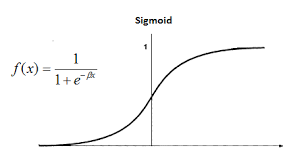
\includegraphics[width=0.5\textwidth]{figures/sigmoid.png}
    \caption{
      A graph of a sigmoid function in 2 dimensions. }
    \label{Figure 1}
  \end{center}
\end{figure}

In this case, as $p \to 1$, the higher the probability we have that this vector is a part of class 1.  

Like in other Machine Learning models, we need to find the optimal parameters.  We turn to maximum likelihood and defining a form of loss that we hope to minimize.  Note, each vector $\mathbf{x}_i$ has an associated class label $y_i$ and $p_i = P(\mathbf{x}_i | \mathbf{w})$.  

Our likelihood function is:  

$$
L = \prod_i p_i^{y_i} (1 - p_i)^{ 1- y_i}
$$

Our loss function is therefore: 

\begin{equation}
\mathcal{L} = - \log P(\text{ data } | \mathbf{w}) = - \sum_i y_i \log p_i + (1 - y_i) \log( 1 - p_i)
\end{equation}

This simplifies to:

$$
\Rightarrow  - \sum_i y_i \log p_i + \log ( 1 - p_i ) - y_i \log(1 - p_i) = - \sum_i y_i \log \frac{p_i}{ 1 - p_i} + \log ( 1 - p_i) 
$$

$$
\mathcal{L}  = - \sum_i y_i \mathbf{w} \cdot \mathbf{x}_i - \log ( 1 + e^{\mathbf{w} \cdot \mathbf{x}})
$$

We need to find the optimal $\mathbf{w}$, so we'll turn to some basic calculus: 

$$
\frac{ \partial \mathcal{L}}{\partial w_k} = - \sum_i y_i x_{ik} - \frac{e^{\mathbf{w} \cdot \mathbf{x}_i } x_{ik}}{1 + e^{\mathbf{w} \cdot \mathbf{x}_i }}  = 0
~~~ w_k \text{ is the kth component of the vector} \mathbf{w}
$$

For each component of the vector w, we have a transcendental equation which has no closed form solution.  

We turn to gradient descent, and have the following update equations: 

$$
\mathbf{w} \leftarrow \mathbf{w} - \eta \frac{ \partial \mathcal{L}}{\partial \mathbf{w}}  ~~ \Rightarrow ~~ 
\mathbf{w} \leftarrow \mathbf{w} + \eta \mathbf{x}^T( y - \text{prediction})
$$

In Naive Byaes we estimate all the w's as independent from each other but in logisitic regression the w's are dependent.  
Logistic Regression won't have an over confidence problem like Naive Bayes has.  

\pagebreak
\subsubsection{Regularized Logistic Regresssion}

If we want to prevent overfitting and prevent the components in our vector of parameters $w$ from getting to big, we can constrain our loss function by doing the following: 

\begin{equation}
\mathcal{L} = - \sum_i y_i \log p_i + (1 - y_i) \log( 1 - p_i) + \frac{1}{2} \lambda^2
\end{equation}

Again finding the optimal value of this expression gives us the following:  

$$
\frac{ \partial \mathcal{L}}{\partial w_k} = - \sum_i (y_i - p_i)y_{ik} +\lambda w_{k} = 0
$$

We get the following new update equations in our gradent descent algorithm: 

$$
w_k \leftarrow w_k - \eta \frac{\partial x}{\partial w_k} \Rightarrow
w_k \leftarrow w_k + \eta \sum_i (y_i - p_i)x_{ik} - \lambda w_k
$$

\begin{equation}
w_k \leftarrow (1 - \eta \lambda) w_k + \eta \sum_i (y_i - p_i)x_{ik}
\end{equation}

We are essentially shrinknig our weight before we move against the gradient.  


\section{ Model Evaluation}

This section focuses on developing new ideas/measurements and evaluation techniques to better understand the performance of our classifier.  \\

Last time we saw the following definitions of accuracy and calibration: 

\textbf{Accuracy: } Fraction of times you predict the correct label. $\frac{1}{N} \sum_i \mathbf{1}(y_i = f(x_i) )$

\textbf{Calibration: } how often does a event with predicted probability $p$ occur?  

The motivation behind moving beyond the accuracy metric is that in general datasets are heavily imbalanced and this can heavily skew percentages.  

We were presented with the confusion matrix which looks like the following figure: 


\begin{figure}[ht]
  \begin{center}
    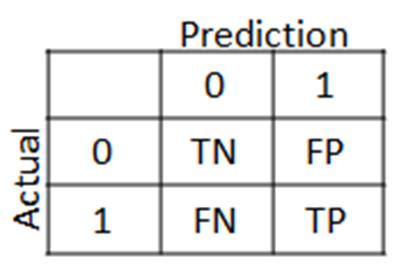
\includegraphics[width=0.5\textwidth]{figures/confusion_matrix.png}
    \caption{
      A confusion matrix. \textit{Source: https://computersciencesource.wordpress.com/2010/01/07/year-2-machine-learning-confusion-matrix/}}
    \label{Figure 2}
  \end{center}
\end{figure}

\pagebreak

The variables in the confusion matrix stand for the following:  

\begin{itemize}
\item \textbf{True Positive (TP): }  We predict 1 while the class is actually 1 i.e we predict a class accurately to be positive when it is actually 1. 

\item \textbf{False Positive (FP): } We predict 1 while the class is actually 0 i.e we incorrectly predict a class to be positive when it is in fact positive.  

\item \textbf{True Negative (TN): } We predict 0 while the class is actually 0 i.e we correctly predict a class is negative (part of class 0). 

\item \textbf{False Negative (FN): } We predict 0 while the class is actually 1 i.e we incorrectly predict a class that is in fact in class 1 or positve as negative or in class 0.  

\end{itemize}
With this concept in mind, we defined some more terms: 

\begin{itemize}
\item \textbf{Precision: } Fraction of positive predictions that are true 
$$\text{Precision } =  \frac{\text{TP}}{\text{TP} + \text{FP}}$$

\item \textbf{True Positive Rate (TPR): } also known as sensitivity, hit rate, and recall is defined as
$$
\text{TPR} = \frac{\text{TP}}{\text{TP} + \text{FN}}
$$
This metric corresponds to the proportion of data points that were correctly classified as positive with respect to all positive points.The higher TPR, the fewer positive points our classifier will miss.

\item \textbf{False Positive Rate (FPR): } also known as fall-out

$$
\text{FPR} = \frac{\text{FP}}{\text{FP} + \text{TN}}
$$
The proportion of negative points that were incorrectly classified as positive with respect to all negative points.  The higher the FPR, the higher we will misclassify negative points.  
\end{itemize}

A high recall classifier can get all the spam thats there but also will tag a lot of legitimate email as spam.  
Highprecision means low recall which is opposite from low precision and high recall.  

\pagebreak

\subsubsection{ROC Curve}
If we vary our threshold and plot the false positive rate against the true positive rate, we develop the ROC curve, which stands for Receiver Operator Characteristic curve.  The AUC or Area Under the Curve is equivalent to accuracy for balanced classification.  

A ROC curve for a really really good classifier might look like this:  

\begin{figure}[ht]
  \begin{center}
    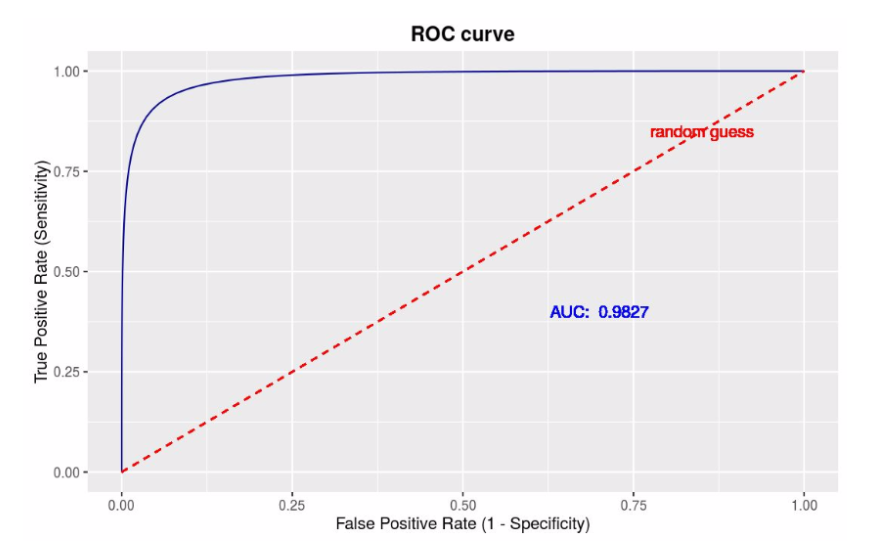
\includegraphics[width=0.5\textwidth]{figures/ROC_curve.png}
    \caption{
      A confusion matrix. \textit{Source: https://github.com/Columbia-Intro-Data-Science/APMAE4990} 
      }
    \label{Figure 3}
  \end{center}
\end{figure}

For more information please see the github link in the figure description, under the lectures directory.  


\section{Computational Social SCience: Exciting Progress and Future Challenges}
This talk was given by Duncan Watts who is the author of \textit{6 Degrees: Living in a Connected World} as well as other books and currently principal research scientist at Microsoft Research.  He was a professor in Sociology in Columbia from 2000 to 2007.  

\begin{itemize}

\item social phenomena arise when individuals interact to produce collective behavior (agents of these systems can vary: individuals, compaies, nationes, etc. ).  People comprise these agents at the end of the day and their interactions affect Macro phenomena.  There is a micro-macro relationship that is extremely difficult to understand and quantify.  
\item This has led to an emerging field of Computational Social Science due in large part by the upsurge of big data from web interactions.  There has been a dramatic increase in scale, scope, and granularity of data.  
 \begin{itemize}
 \item search, buy, produce, consumption $\Rightarrow$ digital exhaust/bread crumbs
 \item the result of all this technological development and digital bread crumbs is computational social science (CSS)
 \end{itemize}
\item outline of the talk.  a) illustrate CSS with two types of examples, social contagion with big data and small data with virtual labs - can run experiments online (b) emerging difficulties

\end{itemize}

\subsection{Social Contagion using Big Data}
a contagion implies large multi-scale, multi-step, peer-to-peer spread and multi-generational branching process (Diffusion, Going Viral, ebola virus)

 \begin{itemize}
 \item usually a S shaped curve implies diffusion but there are lots and lots of models that generate S shaped curves so there are two principal problems here.  1) could result from many processes and 2) typically, our observation of these processes is only for successful diffusive events.  This motivates a strong understanding of unsuccessful attempts of diffusion.  
 
 $\Rightarrow$ the web potentially resolves this problem
 How diverse is going viral?  
 What does viral diffusion look like? 
 Can we predict it? 
\end{itemize}

\subsection{Online Diffusion Project}
\begin{itemize}
\item this project involved created 6 seemingly unrelated projects conducted over the past few years all of which were designed to go viral.  They were in different domains which was important and the goal was to see if there were any patterns in the diffusion.  

They ultimately found that diffusion is of course a rare event but that the structure of diffusion is highly similar from one event to another event.  There was a lot of consistency in terms of the most common structures.  
\end{itemize}

\subsection{Viral or Just Popular - Structural Virality Project}
\begin{itemize}
\item Big data helps to study rare events.  fore each event, one can quantify its structural virality.   Shortest paths range from 2 to $\log(N)$

For popular events, one can ask, what diversity do we see with respect to structure? 
what is the relationship between size and structural virality? 

\item they found an incredible diversity of structural virality and that a popular event is not necessarily viral (broadcasting effect e.g Superbowl isnt a viral event)
\item popularity is driven mostly by the size of the biggest broadcaster.  Indiviudal people can broadcast (celebrity effect)
\end{itemize}


\subsection{How predictable are cascades?}
\begin{itemize}
\item What features drive cascade size?  
\item Goal is to predict final number of retweets of tweets with URLs.  Restrit to 100 per domain

\item features: content, user, content-user interaction $\Rightarrow$ user features are much more predictive than content (interactions add nothing really)

performance asymptotes around 4 (basis of potential existence of a limit)

suggests that predictive accuracy may be subject to some fundemental limit

\end{itemize}
 

\subsection{Virtual Lab}
Social media limits the types of questions one can ask.  Virtual labs try to tackle more tradiitonal challenges of physical labs such as problems like realism, duration and scale. 




















\end{document}

%%% Local Variables:
%%% mode: latex
%%% TeX-master: t
%%% End: